% SH2 Project Report

\documentclass[12pt]{report} % use larger type; default would be 10pt

%%% PAGE DIMENSIONS
\usepackage{geometry} % to change the page dimensions
\geometry{a4paper} % or letterpaper (US) or a5paper or....
\geometry{margin=1in} % for example, change the margins to 2 inches all round

\usepackage{graphicx} % support the \includegraphics command and options
%\usepackage[parfill]{parskip} % Activate to begin paragraphs with an empty line rather than an indent

%%% PACKAGES
\usepackage{booktabs} % for much better looking tables
\usepackage{array} % for better arrays (eg matrices) in maths
\usepackage{paralist} % very flexible & customisable lists (eg. enumerate/itemize, etc.)
\usepackage{verbatim} % adds environment for commenting out blocks of text & for better verbatim
\usepackage{subfig} % make it possible to include more than one captioned figure/table in a single float
\usepackage[utf8]{inputenc} % set input encoding (not needed with XeLaTeX)
\usepackage{fixltx2e}
\usepackage{float}
\usepackage{hyperref}
\usepackage{wrapfig}
%\usepackage{mathtools}
\usepackage{amsmath}
\usepackage[hypcap]{caption}
\usepackage{lipsum}
\usepackage{natbib}
\usepackage{indentfirst}
\usepackage{textcomp}
\usepackage{multirow}

\usepackage{listings}
\usepackage{color} %red, green, blue, yellow, cyan, magenta, black, white
\definecolor{mygreen}{RGB}{28,172,0} % color values Red, Green, Blue
\definecolor{mylilas}{RGB}{170,55,241}


\usepackage[font={footnotesize}]{caption}

\usepackage[labelfont=bf]{caption}

\usepackage{parskip}
\setlength\parindent{20pt} % sets indent to zero
\setlength{\parskip}{5pt} % changes vertical space between paragraphs

%%% HEADERS & FOOTERS
\usepackage{fancyhdr} % This should be set AFTER setting up the page geometry
\pagestyle{fancy} % options: empty , plain , fancy
\renewcommand{\headrulewidth}{0pt} % customise the layout...
\lhead{}\chead{}\rhead{}
\lfoot{}\cfoot{\thepage}\rfoot{}

%%% ToC (table of contents) APPEARANCE
\usepackage[nottoc,notlof,notlot]{tocbibind} % Put the bibliography in the ToC
\usepackage[titles,subfigure]{tocloft} % Alter the style of the Table of Contents
\renewcommand{\cftsecfont}{\rmfamily\mdseries\upshape}
\renewcommand{\cftsecpagefont}{\rmfamily\mdseries\upshape} % No bold!

%%% END Article customizations

%% The "real" document content comes below...

\begin{document}

\begin{titlepage}

\newcommand{\HRule}{\rule{\linewidth}{0.5mm}} % Defines a new command for the horizontal lines, change thickness here

\center % Center everything on the page
 
%----------------------------------------------------------------------------------------
%	HEADING SECTIONS
%----------------------------------------------------------------------------------------

\textsc{\LARGE The University of Edinburgh}\\[1.5cm] % Name of your university/college
\Large Senior Honours Project Report \\[0.5cm] % Major heading such as course name
\textsc{\large BSc GEOPHYSICS}\\[0.5cm] % Minor heading such as course title

%----------------------------------------------------------------------------------------
%	TITLE SECTION
%----------------------------------------------------------------------------------------

\HRule \\[0.4cm]
{ \huge \bfseries Improving the prediction of magnetic disturbances from solar wind parameters}\\[0.4cm] % Title of your document
\HRule \\[1.5cm]
 
%----------------------------------------------------------------------------------------
%	AUTHOR SECTION
%----------------------------------------------------------------------------------------

\begin{minipage}{0.4\textwidth}
\begin{flushleft} \large
\emph{Student:}\\
Kittiphon \textsc{Boonma} % Your name
\end{flushleft}
\end{minipage}
~
\begin{minipage}{0.4\textwidth}
\begin{flushright} \large
\emph{Supervisor:} \\
Dr.Brian \textsc{Hamilton} % Supervisor's Name
\end{flushright}
\end{minipage}\\[4cm]

%----------------------------------------------------------------------------------------
%	DATE SECTION
%----------------------------------------------------------------------------------------

{\large 04/04/2014}\\[3cm] % Date, change the \today to a set date if you want to be precise

%----------------------------------------------------------------------------------------
%	LOGO SECTION
%----------------------------------------------------------------------------------------


\includegraphics[width=0.2\textwidth]{./UoE_Geosciences}% Include a department/university logo - this will require the graphicx package
 
%----------------------------------------------------------------------------------------

\vfill % Fill the rest of the page with whitespace

\end{titlepage}


%----------------------------------------------------------------------------------------
%	ABSTRACT
%----------------------------------------------------------------------------------------
\begin{abstract}

Magnetic indices are used as a measure of the intensity of various geomagnetic activities. Dst index measures the strength of the equatorial Ring Current. A previous study by \cite{newell07} proposed a function, $d\Phi_{MP}/dt$, which is said to give the best correlation between the solar wind parameters and the geomagnetic indices. The coupling function $E_{SR}$ was claimed to be the second best. This study aims to investigate these claims by applying corrections to indicies and using new data (2000-2013) which the previous study did not have. Dst index measures both the ring current (Est index), and the induced current in the conducting Earth (Ist index). This gives rise to the idea of improving the prediction model of the geomagnetic disturbances by replacing the Dst index with Est index, and the Ist is eliminated because it is produced indirectly by the solar wind parameters.  The analytical results from this study confirms that the correlation between the top coupling function with Dst can be improved by replacing it with Est index. However, this is not the case for the second best function, $E_{SR}$. An additional hypothesis is that the measure of auroral electrojet indices, AU and AL, contain contributions from the ring current. The results from the investigation confirmed the hypothesis since about  $8\%$ of the AU index and  $6\%$ of the AL index were the contribution from the x-component of the ring current. Removing the effect of ring current improves AU index but worsens AL index. Overall, since the claimed top function $d\Phi_{MP}/dt$ was not consistently better than $E_{SR}$ when changes were introduced, $d\Phi_{MP}/dt$ function may not be as robust and correlate best with every indices as \cite{newell07} claimed it to be.


\end{abstract}
%----------------------------------------------------------------------------------------

%----------------------------------------------------------------------------------------
%	TABLE OF CONTENT
%----------------------------------------------------------------------------------------


\tableofcontents

%----------------------------------------------------------------------------------------


%%%%%%%%%%%%%%%%%%%%%%%
%% PROJECT CONTENT STARTS HERE%%%%
%%%%%%%%%%%%%%%%%%%%%%%


\chapter{Introduction} \label{chap:introduction}
\vspace{-10pt}
The monitoring and accurate prediction of magnetic disturbances in the Earth's upper atmosphere, the ionosphere and the magnetosphere, has become increasingly important due to the expansion of human activity at high altitudes, in space, and on the ground where sensitive technologies, such as power grids and directional drilling for oil and gas, can be affected.  Understanding the coupling mechanisms and how the solar wind affects the Earth's magnetic field is crucial. Therefore, it is necessary to quantitatively assess the underlying statistical and correlating models. 

Geomagnetic indices represent a measure of geomagnetic activity, which is a key signature of how the Earth's ionosphere and magnetosphere respond to interactions with the solar wind. There are many types of indices, each describing different geomagnetic activity, and many try to isolate the activity from different sources (current systems) in the ionosphere/magnetosphere. For the past 15 years in the field of Solar Terrestrial studies, these indices have become a key parameter in detecting and describing space weather events.

The overall aim of this study is to investigate the improvements on geomagnetic indices (Dst, Est, AU, and AL) and their ability to be predicted by the solar wind parameters. There are three parts to the investigation:

\begin{description}
  \item[1)] The first hypothesis is that it may be more appropriate to predict the Est index, rather than the Dst index (as many scientists have done in the past). The correlation between the indices and a coupling function is used to test this hypothesis. 
  
  \item[2)] We investigate the possibility of improving the AU and AL indices by subtracting contaminating effects arise from the ring current. Again, using coupling functions, it can be tested whether the corrected AU and AL indices have a stronger correlation than the original indices. 
  
  \item[3)] A study previously done by \cite{newell07} has found a good correlation with the Dst index (and many others) and claimed that $d\Phi_{MP}/dt$ is the best coupling function.The analysis from this study will be used to test if the claim stands up to scrutiny, especially with the new data (up to 2013) which \cite{newell07} did not have. The corrected indices will also be used to test the claim, and the investigation will extend into looking at  the second best coupling function $E_{SR}$ (claimed by \cite{newell07}) as well. 
\end{description}
  \noindent This chapter introduces the reader to the project and the underlying physical background. The analytical methods are presented in Chapter~\ref{chap:method} (p.~\pageref{chap:method}). The results and corresponding discussions are presented in  and Chapter~\ref{chap:results}(p.~\pageref{chap:results}). The overall discussion and conclusion will be presented in Chapter~\ref{chap:discussion}(p.~\pageref{chap:discussion}).
    
\begin{figure}
\centering
 \vspace{0pt}
    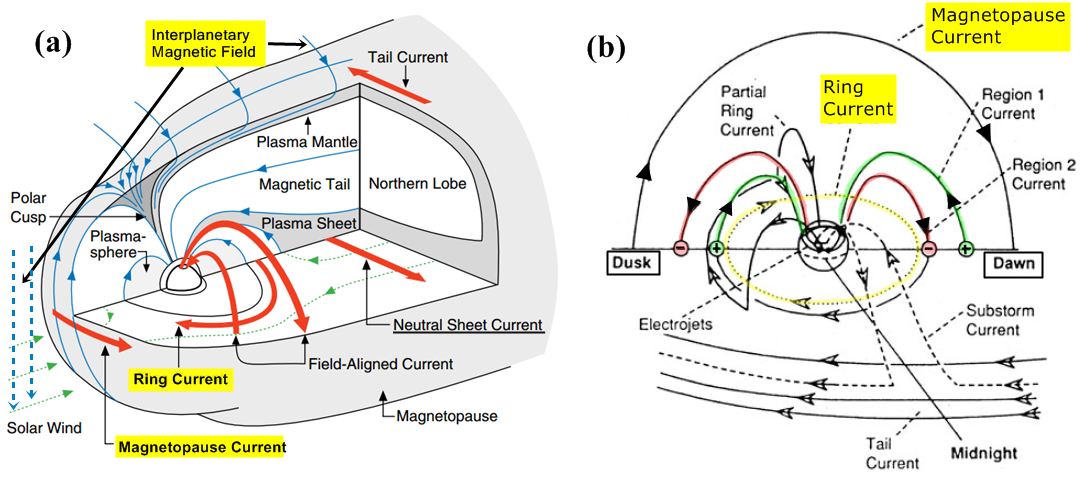
\includegraphics[width=1.05\textwidth]{./magnetosphere}
 \vspace{0pt}
  \caption{(a) A diagram of the magnetosphere showing the current systems and plasma regions (Source: \cite{russell00}). (b) A diagram of a cross-section of the outer magnetosphere, looking towards the Sun. The diagram represents various current systems within the magnetosphere-ionosphere cavity, which give rise to magnetic activity  (Source: Modified from \cite{mcpher95}).} \label{fig:magnetosphere}
   \vspace{5pt}
\end{figure} 
\vspace{-10pt}
\section{Solar wind and Magnetosphere} \label{sec:solarwind}
\vspace{-5pt}
Other than solar radiation, solar wind is regarded as the second most crucial connection between the Earth and the Sun. The \emph{solar wind} is defined as a stream of ionized particles ejected from the Sun. Within the solar wind stream, there is an embedded \emph{Interplanetary Magnetic Field (IMF)}(Figure~\ref{fig:magnetosphere} (a)) which the solar wind carries through the solar system. The solar wind carries this weak magnetic field past the magnetized Earth, where it controls the strength of the coupling between the upper atmosphere (magnetosphere and ionosphere) and the solar wind.
	
As the Earth travels around the Sun in this dynamical solar-wind environment, the Earth's magnetic field interacts with the solar flux. The blast of solar wind envelops and deflects around the Earth's dipole geomagnetic field, compressing the magnetosphere to 11 Earth-radii (\textit{R\textsubscript{e}}) on the dayside, and stretches the magnetosphere outwards into a long tail, far past the Moon's orbit (60\textit{R\textsubscript{e}}) on the nightside \citep{campbell03}.
	
The energy, plasma, and momentum are transferred from the solar wind into the Earth's upper atmosphere through the merging of the Earth's magnetospheric field lines and the IMF. The magnetopause (Figure~\ref{fig:magnetosphere} (a)) is the boundary between the Earth's magnetic field and the solar wind. The merging process occurs within the magnetopause, however, the merging location depends  on the orientation of IMF \citep{russell00}.
	
Figure~\ref{fig:gsm} shows the \emph{Geocentric Solar Magnetospheric (GSM)} coordinate system which is typically used when dealing with the orientation of IMF. B\textsubscript{x} lies along the Earth-Sun plane and is positive towards the Sun. B\textsubscript{y} is the cross product of the magnetic dipole B\textsubscript{z} and  B\textsubscript{x}, and B\textsubscript{z} represents the cross product of B\textsubscript{x} and B\textsubscript{y}. It is considered the best coordinate system for the study of the effect of IMF components on the magnetospheric phenomena because by applying this system, the direction of the Earth's geomagnetic field near the `nose' of the magnetosphere is well-ordered. This coordinate system is also applied to the components of the field used to calculate the IMF clock angle in section ~\ref{sec:dphi}.
	
\noindent There are two scenarios in which the IMF can merge with the Earth's magnetic field, both of which are illustrated by the Dungey's Model in Figure~\ref{fig:imf}:
\vspace{10pt}

\begin{enumerate}
 \item Figure~\ref{fig:imf} (a) shows the case where IMF is directed southward ({\bfseries B\textsubscript{z}$<$0}), and the dayside shrinks by flux ablation. According to the Dungey's Model, with this configuration, the reconnection occurs with closed magnetospheric field lines on the dayside magnetopause. This leads to the formation of the opened field lines, which are dragged by the magnetic tension away from the Sun. On the dayside, the energy flows from the magnetic field into the plasma, however, there is some electromagnetic energy flux at the tail, and this energy flows from the plasma into the magnetic field \citep{russell00}. 
 
 The energy transferred into the magnetic field is stored as magnetic energy in the magnetotail \citep{men11}. This stored energy can be released from the tail randomly during violent bursts of energy, called \emph{substorms}, and causes the plasma to flow into the magnetosphere. The field and plasma continue to move towards the reconnection point on the dayside, as shown by the green dashed line in Figure~\ref{fig:magnetosphere} (a), and the cycle is repeated.
  
 \item  Figure~\ref{fig:imf} (b) illustrates the situation when IMF is directed solely northward ({\bfseries B\textsubscript{z}$>$0}), and the dayside grows by flux accretion. In this case, the reconnection still occurs, however, the effect on the magnetosphere will be different from the previous case. The reconnection occurs with opened magnetospheric field lines tailward of the cusp (Figure~\ref{fig:magnetosphere} (a)). 
 
 However, the northward-IMF model is not consistent with the results from previous studies on electron data and on solar proton data. Therefore, it is important to note that it is highly doubtful that the same field line would connect to both the north and south neutral points at the tail \citep{russell72}.

\end{enumerate}
\vspace{15pt}

 To put this into context, these merging events illustrate the physical processes of how the solar wind continually feeds energy into the Earth's atmosphere \citep{russell00} and affects the magnetosphere and ionosphere. Ultimately, this produces the disturbances which are measured by the indices studied in this project. Therefore, it is justifiable and appropriate to consider solar wind based coupling functions (Section~\ref{sec:couplingfunctions}). The northward directed IMF usually causes less disturbance and, hence, smaller indices. This explains the importance of the clock angle term (Equation~\ref{eq:thetac} in the coupling functions.
	
\begin{figure} 
\centering
 \vspace{-20pt}
    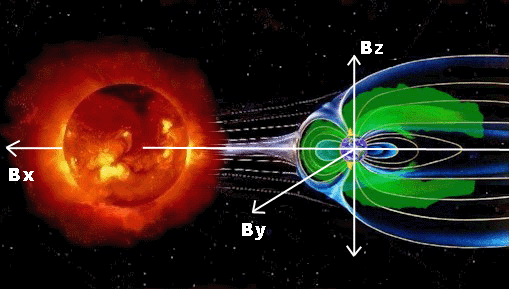
\includegraphics[width=0.8\textwidth]{./gsm}
 \vspace{5pt}
  \caption{Diagram showing the \emph{Geocentric Solar Magnetospheric (GSM)} coordinate system. x-axis is Earth-Sun line and is positive towards the Sun. y-axis is the cross product of the magnetic dipole axis and the x-axis. z-axis is the cross product of x- and y-axes. (Source: http://poleshift.ning.com)} \label{fig:gsm}
   \vspace{5pt}
   
   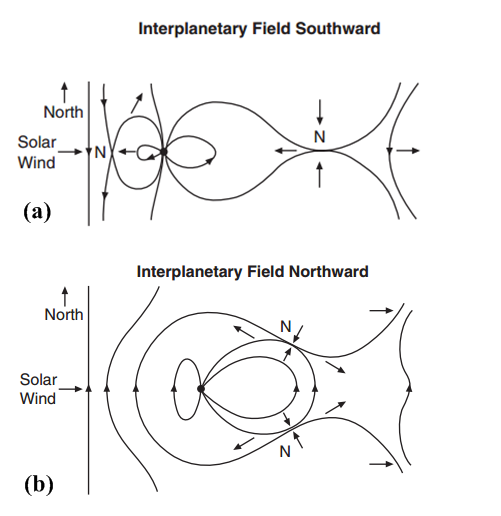
\includegraphics[width=0.8\textwidth]{./imf}
 \vspace{0pt}
  \caption{\emph{The Dungey's Model of the Magnetosphere} showing the interaction between the solar wind Interplanetary Magnetic Field (IMF) and the Earth’s magnetosphere. `N' represents the reconnection area which is also known as Neutral point. (a) A schematic illustration of the open magnetosphere and the reconnection theory with IMF pointing southwards and the Earth’s field pointing northward. (b) A schematic illustration of the closed magnetosphere with both IMF and Earth’s magnetic field pointing northward.(Source: \cite{russell00})} \label{fig:imf}
\end{figure} 
\vspace{-10pt}
\section{Current Systems}
\vspace{-10pt}
There are several current systems in the upper atmosphere that magnetic perturbations can originate from. This study is mainly concerned with two current systems, both of which are described in this section. 

\subsection{Magnetopause Current}

There are several sources of electric currents co-existing within the magnetosphere-ionosphere system. They can be either directly or indirectly associated with the dynamical interaction between the Earth's environments and the Sun \citep{men11}. This study mainly focuses on the currents arising from the interaction between the Earth's magnetic field and the solar wind. One of the current systems, namely \emph{Magnetopause Current}, will be described in this section. 

 The \emph{Magnetopause Current}, or also known as `\emph{Chapman-Ferraro Current}', is the basic nature of the interaction between the Earth's magnetic field and the solar wind. The existence of such a current system was first deduced in 1930's by Sydney Chapman and Vincenzo Ferraro \citep{chapfer31}. Magnetopause represents a surface of current layer (Figure ~\ref{fig:magnetosphere} (a)), and separates the solar wind (high density, low magnetic fields ({\bfseries B})) from the magnetosphere (low density, high magnetic fields ({\bfseries B})). In the first approximation, magnetopause forms at a distance of about 8-11 \textit{R\textsubscript{e}}where the magnetic pressure of the Earth's field equals the dynamic pressure of the solar wind \citep{men11}. As the solar wind particles begin to penetrate the magnetopause they experience the Lorentz force provided by the magnetopause current, which deflects the electrons and protons of the solar wind in opposite directions normal to the field,  shielding the Earth's magnetic field from the solar wind. This magnetopause current, shown in Figure~\ref{fig:magnetosphere} (b), flows towards \emph{dusk} on the dayside, and towards \emph{dawn} on the nightside magnetopause where it is called the \emph{tail current} (Figure~\ref{fig:magnetosphere} (b)). A type of current called the \emph{Neutral Sheet Current} flows duskward in the magnetic equatorial plane and acts as a barrier confining the tail part of the magnetopause current inside the magnetosphere (Figure~\ref{fig:magnetosphere} (a)). From the right-hand rule, it can be speculated that the ground magnetic field will be affected by a southward perturbation. The magnetopause current is important to this study because it is used in the correction of the Dst index in Section~\ref{sec:dphi}.
 
\subsection{Ring-current} \label{sec:ring}
 
Ring current is produced from the eastward drift of electrons and the westward drift of protons in a ring around the magnetic equator of the Earth at a distance of $3-5$ \textit{R\textsubscript{e}} (Figure~\ref{fig:magnetosphere}), where the magnetic field is approximately dipolar \citep{men11}. \cite{burton75} used what was understood, regarding the control of the reconnection process of IMF, to demonstrate that the ring current could be predicted from solar wind parameters. The amount of convected southward IMF is proportional to the injection rate of the energy that goes into the ring current \citep{le04}. Similar to the tail current, the ring current flows duskward on the Earth's magnetic equatorial plane, and by applying the right-hand rule, its ground effect is the reduction in the main field strength at low latitudes due to the southward perturbation. This is similar to the effect of the magnetopause current. 

For the purpose of this study, ring current is important because its strength directly varies in response to the solar wind. Since the ring current is associated with the solar wind-magnetosphere interaction, the solar wind parameters can be studied through Dst index, which measures the strength of the ring current. 

\begin{figure}
\centering
 \vspace{-5pt}
    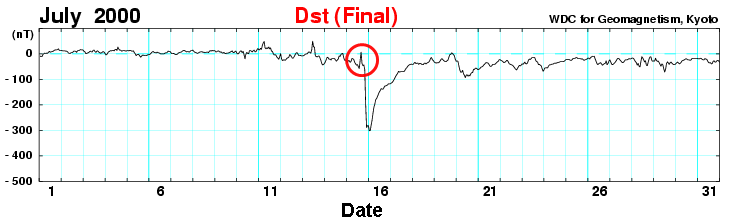
\includegraphics[width=1\textwidth]{./dst}
 \vspace{-15pt}
  \caption{A graph showing Hourly Equatorial Dst Values of July 2000. The y-axis is the H-component of the field, while the x-axis represents each day of the month. The increase in Dst (circled) amplitude prior to a large drop is a result of magnetospheric compression. The large decrease in Dst amplitude signifies the main phase of the storm. (Source: World Data Centre for Geomagnetism, Kyoto)} \label{fig:dst}
   \vspace{0pt}
\end{figure} 

\section{Geomagnetic Indices}
 \vspace{-5pt}
\subsection{Disturbance Storm Time (Dst) Index} \label{sec:dst}
 \vspace{-5pt}
During a period of intense solar activity, the southward IMF that merge with the Earth's magnetic field can be strong and have long duration. The reconnection occurs at the `nose' of the magnetosphere (Figure~\ref{fig:imf} (a)) and causes compression of the magnetosphere on the day side and continues down the tail. This compression distorts the Earth's dipole field and provides an entry for the solar wind particles, which cause the geomagnetic disturbances i.e. geomagnetic storms. These storms are the main source that provide energy for the ring current (Section~\ref{sec:ring}) which has a westward-flowing current. This westward current causes a horizontal (H)-component field depression worldwide \citep{campbell03}. 

Disturbance Storm Time index (Dst) is one of many geomagnetic indices. It monitors the magnetic storm level worldwide, as well as representing the axially symmetric magnetic disturbance at the dipole equator on the Earth's surface \citep{men11}. Dst index is derived from averaging the H-component of the Earth's magnetic field from well-spaced mid- or low-latitude observatories  from all over the world. 

The severity of the geomagnetic disturbance is represented by the magnitude of the decrease in H-component field, i.e. the disturbance field is southward. An example of Dst data is shown in Figure~\ref{fig:dst}. The circled area emphasizes a sharp increase prior to a large drop in amplitude, which is caused by the compression of the magnetosphere, and the following drop after the upward spike is caused by the ring current.

The derivation of Dst described in this section is based on  \cite{sugi91}. 
At a time `$t$', the $Dst(t)$ is defined as the average of the disturbance variation of H-component of the field, $D_i(t)$, at `n' observatories. In order to normalize the Dst index to the dipole equator, the expression is divided by the average of the cosines of magnetic dipole latitudes of the \textit{i}-th observatory, $\lambda_i$. Thus, $Dst$ can be expressed as: 
\begin{align}
Dst (t) =\sum_{i=1}^{n} D_i (t)  / \sum_{i=1}^{n} \cos(\lambda_i) \label{eq:1}
\end{align}
\noindent For further technical details and in-depth derivation, the reader is referred to \citep{sugi91}.
Many previous studies (\cite{russell74}, \cite{bik12}) have been done in attempt to correlate the Dst index, and therefore the ring current strength, with the solar wind parameters such as the bulk plasma speed, strength, and the orientation of the magnetic field that it carries. This project investigates if the correlation could be improved by replacing it with the Est Index. 

\vspace{-10pt}
\subsection{Est and Ist Indices} \label{sec:estist}
\vspace{-5pt}
 Geomagnetic field disturbances are commonly thought to be caused solely by a field source outside of the Earth's body. However, it has recently been found that a sole external field source may not always be the case. The disturbance magnetic field representations have some difficulties due to the \emph{secondary field}, which arises from the external time-varying source field inducing electric currents in the Earth. The strength of this secondary field is approximately one third of the inducing field \citep{maus04}. Thus, the field disturbance observed on the Earth's surface and measured by $Dst$ index is, in fact, the sum of the external source field and its induced counterpart. 
 
 A physically correct representation of the symmetric disturbance field is provided by the \emph{internal} and \emph{external} contributions, which are derived by taking a Fourier transform of the $Dst$ index as well as implementing a conductivity model \citep{utada03}. Therefore, the $Dst$ index can be split into the {\bfseries external dipole source field} (\emph{Est Index}) and the {\bfseries internal induced dipole field} (\emph{Ist Index}). Thus, at any given time;
\begin{align}
Dst (t) = Est (t) + Ist (t) \label{eq:2}
\end{align}
\noindent and the corresponding internal and external dipole fields are represented as
\begin{align}
\mathbf{B}_{ext} (t) = - Est(t) \Big (\sin \theta \hat{\theta} - \cos \theta \hat{r}\Big ) \label{eq:3} \\
\mathbf{B}_{int} (t) = - Ist(t) \Big ( \sin \theta \hat{\theta} + 2 \cos \theta \hat{r}\Big ) \label{eq:4} 
\end{align}
\noindent where $\hat{\theta}$ is the a unit vector for the local southward, and $\hat{r}$ is the local outward unit vector. The negative signs in Eqn.~\ref{eq:3} and ~\ref{eq:4} are present because $Dst$ represents the northward field, while $\hat{\theta}$ points southward. In an ideal conductor, the strength of the induced field would have its radial component cancelling out the radial component of the inducing field on its surface. However, in the case of the real Earth, the amplitude and phase lag relation between the induced internal and induced external field depends on the \emph{frequency content} of the external source field \citep{maus04}. For more mathematical details on separating external and internal parts of the symmetric disturbance field, the reader is referred to \cite{maus04}. $B_{ext}$ and $B_{int}$ will be used later in this project (Section~\ref{sec:correctaual}) for the correction of the AU and AL indices, which will be described next.
\vspace{-10pt}
\subsection{Auroral-Electrojet (AE) Indices}\label{sec:ae}

The Auroral-Electrojet (AE) indices were introduced as a measure of global disturbances resulting from the auroral electrojet activity, and thus specifying the state of the Earth's upper atmosphere. It should be noted that the term ``AE Indices'' includes the \emph{AU} and \emph{AL} indices, which this study will also focus on,  whereas the term ``AE Index'' is just the AE index itself. AE indices data are maintained at the World Data Center for Geomagnetism in Kyoto, Japan, and  has been exploited both qualitatively and quantitatively as a correlation index in the fields of radio propagation, substorm morphology, the behaviour of communication satellites, and the magnetosphere-IMF coupling.

The AE indices are derived from the geomagnetic variations in the horizontal component (H) of the main field observed at the selected observatories along the auroral zone in the northern hemisphere. The variations are measured from a baseline, which is determined for each individual observatory, and then go through a normalization process. For more detail of the normalization process, please refer to \cite{men11}. 

In a superimposed plot of one-minute H values from all the AE observatories at each given universal time (UT) the AU index represents the upper envelope of the plotted points, while the AL index represents the lower envelope. The AE value gives the separation of these envelopes:
\begin{align}
AE = AU -AL \label{eq:5}
\end{align}
The AU and AL indices are defined by the largest and the smallest values respectively, selected from the data from all the stations \citep{men11}. While the AE index represents a measure of global auroral electrojet activity, the AU index is intended to represent a measure of the strongest current intensity of the eastward auroral electrojet, and the AL index represents a measure of a westward auroral electrojet. Some caution should be taken when using the indices for substorm studies for a number of reasons. One in particular, which is relevant to our study, is that although the indices are generated from ionospheric electrojet current, magnetospheric current such as the equatorial ring current can also affect the indices. \cite{davis66} carried out a study and suggested that the negative values of the AU index may have occurred due to the contribution from the ring current. This project will also investigate this speculation to see whether the corrected AU and AL indices (Section~\ref{sec:correctaual}) would correlate with the coupling functions better. 
\vspace{-10pt}
\section{Coupling Functions} \label{sec:couplingfunctions}
\vspace{-5pt}
\subsection {d$\Phi_{MP}$/dt}\label{sec:dphi}
\vspace{-5pt}
The velocity, density, or pressure of the solar wind themselves are unlikely to have much predictive power for the magnetospheric indices. However, it was realized by \cite{dun61} that the IMF is continual and continuously varying, thus, suggesting the importance of $B_z$ and the merging between the IMF and the Earth's fields (Section~\ref{sec:solarwind}). 
There are many different coupling functions representing a variety of magnetospheric activities due to the interaction between the solar wind and the magnetosphere. The one particular  coupling function this project focuses on was proposed by \cite{newell07}. This function represents the rate of which magnetic flux is open to the magnetosphere, and is presented as;
\begin{align}
d\Phi_{MP}/dt = v^{4/3} B_{T}^{2/3} \sin^{8/3} (\theta_c/2) \label{eq:dphi}
\end{align}
\noindent where $v$ is the approximated rate at which IMF field lines approach the magnetopause, $B_T$ is the magnitude of the interplanetary field, and $\sin^{8/3} (\theta_c/2)$ represents the percentage of the merging IMF lines. The IMF clock angle ($\theta_c$), here, is defined by;
\begin{align}
\theta_c = arctan (B_y/B_z) \label{eq:thetac}
\end{align} 
\noindent where $B_y$ and $B_z$ represent the y-component and the z-component of the field in GSM coordinates (Figure~\ref{fig:gsm}). The reader is referred to \cite{newell07} for an in-depth derivation.

The study by \cite{newell07} shows that the AU and AL indices both correlate best with this coupling function. However, the Dst index does not correlate best with just $d\Phi_{MP}/dt$ alone but with an additional factor of $p^{1/2}$, which gives $p^{1/2}d\Phi_{MP}/dt$. The term $p^{1/2}$ was used to correct for the magnetopause currents. This effect was taken into consideration when applying the coupling function to our data set. 

The coupling function $d\Phi_{MP}/dt$ greatly depends on the term involved the IMF clock angle, $\sin^{8/3} (\theta_c/2)$. Despite the awkward 8/3 exponent, which was a result based on `trial and error search' through all the possible values, the dependence of $d\Phi_{MP}/dt$ on the clock angle is rather straightforward. 

The physical meaning of $\sin^{8/3} (\theta_c/2)$ is the fraction of the field lines impacting the magnetosphere which merge and is a function of the magnetic shear. \cite{newell07} also carried out a statistical comparison for the relationship between the IMF clock angle and various coupling functions. All the coupling functions, including the $d\Phi_{MP}/dt$, predicted that the greatest amount of field lines merging is due to the southward IMF (Figure~\ref{fig:imf}), and the functions go to zero for a northward IMF. This can also be used to support the statement that says the southward IMF model is preferable over the northward IMF, as previously discussed in section~\ref{sec:solarwind}.    

 All in all, the coupling function $d\Phi_{MP}/dt$ is chosen by this study because, according to a study done by \cite{newell07}, it gives a reasonable prediction of a variety of magnetospheric phenomena, and is claimed to have the best correlation with every indices (r $>$ 0.80 in some cases). This study will, therefore, investigate the robustness of this function and how it performs when the corrected indices are used. The second best coupling function $E_{SR}$, as claimed by \cite{newell07}, will also be used to test the robustness 


\vspace{-10pt}
\subsection{E$_{SR}$}
 \vspace{-5pt}
This coupling function was proposed by \cite{scurry91} in the study of the transferring of energy into the magnetosphere. The function is represented as;
\begin{align}
E_{SR} = v B_{T} \sin^{4} (\theta_c/2) p^{1/2} \label{eq:esr}
\end{align}
\noindent It examines the relation between the reconnection mechanism and the orientation of the IMF as well as the upstream solar wind parameter. The solar wind parameters required for this coupling function are the same as those used in  $d\Phi_{MP}/dt$. In the study done by \cite{newell07}, $E_{SR}$ gave the second best correlation coefficient for Dst (1995-2002) and the third best for Dst (1984-1994). However, $E_{SR}$ does not correlate well with the AU and AL indices at all. 

In this study, the coupling function $E_{SR}$ is used to test whether the function $d\Phi_{MP}/dt$ really is the best coupling function, as claimed by \cite{newell07}. This investigation will be also be comparing the correlation coefficient between $E_{SR}$ and OMNI 2 data with the results from \cite{newell07}. Only the basic description of this coupling function is given here because it is not the main focus of this study, however, for more details on the $E_{SR}$ function the reader is referred to \cite{scurry91}.

 
 
 

\chapter{Data}
\vspace{0pt}
\section{Solar Wind Parameters, Dst, AU, and AL Data} \label{sec:solardata}
\vspace{0pt}
The solar wind dataset used in this study is called ``OMNI 2'' data and is obtained from NASA's OMNIWeb Data and Service site (http://omniweb.gsfc.nasa.gov) provided by the Space Physics Data Facility (SPDF) at NASA/Goddard Space Flight Center. The OMNI 2 data are a multi-source dataset which contains continuous time-series of solar wind data contributed by several different spacecraft. Most of these spacecrafts are in geocentric orbit, while some are orbiting the Sun at the Lagrange point. Within the data set, factors such as time-delays between satellites at different locations have already been dealt with before the data were published on the site.  

The particular data set that was used in this study is low-resolution with hourly averages from the year 1963 to 2013. The data set has 55 columns, and the information selected for the purpose of this investigation is: 
\begin{table}[h]\small
\centering
\renewcommand{\arraystretch}{1.1}
\begin{tabular}{ l  c}
\hline
  Parameters &Column  \\ \hline
 Year & 1 \\
Decimal Day & 2\\
Decimal Hour & 3 \\
IMF Field Strength, $B_T$ (nT) &10 \\
$B_y$ (nT) & 16 \\
$B_z$ (nT) & 17 \\
Solar wind speed, $v$ (km/s) & 25 \\
Solar wind pressure, $p$ (nPa) & 29 \\
Dst Index (nT) & 41 \\
AL Index (nT) & 53 \\
AU Index (nT) & 54 \\
\hline
\end{tabular}\caption{The column number in which the solar wind parameters are extracted from OMNI 2 data. Note: $B_x$ and $B_y$ are field components in GSM coordinates (Figure~\ref{fig:gsm})} \label{tab:column}
\end{table}

\vspace{-5pt}
\noindent This selected information is then used to calculate the coupling functions, $d\Phi_{MP}/dt$ (Equation~\ref{eq:dphi}) and $E_{SR}$ (Equation~\ref{eq:esr}). Some modifications have to be made on some sets of data, such as Dst, AU, and AL indices, as well as the solar wind pressure. These modifications will be discussed later in Section ~\ref{sec:correction} and ~\ref{sec:timeint}. \par

\vspace{0pt}
\section{Est and Ist Data} \label{sec:est}

In this study, the Est index data would be used to replace Dst in the hope of improving the correlation with the coupling function, and therefore improving the prediction of the magnetic disturbances from solar wind parameters. 

The Est and Ist data were extracted from a set of data obtained from the File Transfer Protocol (FTP) Directory of the National Geophysical Data Center (NGDC) which is a part of the USA's National Oceanic and Atmospheric Administration (NOAA). The dataset contains the data from 1957 - 2013, and has 4 columns with the first column being the Julian date, the second is Dst index values, the third column is the Est index value, and the fourth being the Ist index value. 
\vspace{-5pt}
\section{Correction on Dst Index data} \label{sec:correction}

As mentioned previously in Section~\ref{sec:dphi}, there is an additional factor of $p^{1/2}$ when correlating Dst index with the coupling function.

On the sunward side, the magnetopause is \emph{compressed} and drawn out tailward until the magnetic pressure from the magnetosphere balances the dynamic pressure of the incoming solar wind \citep{russell74}. This leads to the distortion of the magnetosphere, which is associated with the magnetopause currents. Therefore, the Dst index will need to correct for this effect by removing an amount proportional to a value of solar wind pressure ($p$).
 
   Due to this correction, the correlation of the coupling function is not with ``Dst'' but actually with ${\mathbf{Dst - 18.9 p^{1/2}}}$ \citep{newell07}.

\vspace{-5pt}
\section{Time Integration of Solar Wind for Each Index} \label{sec:timeint}

In their study, \cite{newell07}worked with 10 indices, each representing a different magnetospheric phenomena. Therefore, it was expected that the response of these indices to the solar wind would show a variety of timescales and decay with differing hysteresis. So, it became apparent that time-integration is needed, and that the integration time for a given index is somewhat invariant of the coupling function used \citep{newell07}.

 Although this investigation is focusing on the coupling function $d\Phi_{MP}/dt$, time integration process can be applied to other coupling functions as well, such as $E_{SR}$. The coupling function, $d\Phi_{MP}/dt$, was calculated first at an hourly time resolution before the time integration was done.

The process involved separately altering the number of hours of IMF data integrated over, and the weight, $w$ ($0< w <1$), used in the integration.

The \emph{weighted mean} is applied to each hour. The weight takes the form of $w^n$ ( $n$ = the hour before the present), and the number of hour is altered for different indices (Table~\ref{tab:inttable}). Since the present hour influences the indices prediction the most, it is therefore the most weighted ($w^0 = 1$), and the hours following that incrementally increase in $n$ (weighting factor decreases) \citep{newell07}. The solar wind integration time optimizing each index is shown in Table~\ref{tab:inttable}.
  
\begin{table}[h]\small
\centering
\renewcommand{\arraystretch}{1.2}
\begin{tabular}{c c c}
\hline 
  Index  &  No. of Hours of IMF & $w$ \\
 \hline
Dst & 72 & 0.95 \\ 
AU& 3 & 0.77\\
AL & 3 & 0.69 \\
\hline
\end{tabular} \caption{The Solar Wind Integration Time for Each Index} \label{tab:inttable}
\end{table}

\vspace{0pt}
The Dst index, a measure of the ring current, requires the longest solar wind time integration (72 hours) because large ring currents can occur continuously for several days even after dayside merging ceases. This is due to substorm, from the crossing neutral point at the tail of the magnetosphere (Figure~\ref{fig:imf} (a)), injecting energy into the ring current system (refer to section \ref{sec:solarwind}). 

Only 3 hours of solar wind time integration is needed for the AU and AL indices because that is roughly the amount of time it takes for the auroral electrojets (refer to section ~\ref{sec:ae}) to return to their normal state after dayside merging ceases \citep{newell07}.


\chapter{Method}\label{chap:method}
\vspace{-20pt}
The data was processed mainly using MATLAB\textsuperscript{\textregistered}. Some of the codes used throughout this study were written by the student, while some help and Function codes were provided by the project supervisor, Dr. Brian Hamilton (BGS). Several different codes were written since this study investigates the correlation between the coupling functions, $d\Phi_{MP}/dt$ and $E_{SR}$, with different geomagnetic indices. This section will describe the processing steps implemented within different codes. 

\vspace{-10pt}
\section{Main Code} \label{sec:maincode}
\vspace{-10pt}
The main code was written by the student to investigate the correlation between the coupling functions and the indices. The steps implemented in the main code (Appendix~\ref{chap:app}) are used to process different indices and coupling functions, therefore the description of each step is kept as general as possible. The implemented steps are:
\begin{enumerate}
\item The code started by importing the OMNI 2 data and the solar wind parameters needed were extracted. In the case of Est, the code imports the data from the NOAA data set and the Est index values were then extracted.
\item The clock angle ($\theta_c$) was then calculated using the Equation~\ref{eq:thetac}. This is the same for all coupling functions used in this study.
\item The coupling function was calculated using the Equation~\ref{eq:dphi} for $d\Phi_{MP}/dt$, and Equation~\ref{eq:esr} for $E_{SR}$.
\item The OMNI 2 data contains a lot of missing data. The missing data appeared to have very large value such as 99.99 nPa for the solar wind pressure ($p$), 9999 km/s for the solar wind speed ($v$), and 999.9 nT for the IMF field strength ($B_T$), the y-component ($B_y$), and the z-component ($B_z$). Any row of data with at least one missing datum would be marked as a faulty row. 
\item The proceeding 72 or 3 hours (Table~\ref{tab:inttable}) were checked. The selected blocks should have 72 rows for Dst and Est indices, and 3 rows for AU and AL indices. By doing this, data points with the required number of good and complete hours would be selected. Any data points that did not have the required number of good hours preceding them were flagged as bad.
 
\item The time integration of solar wind for the index was then implemented.  The Dst and Est indices are best predicted by integrating over 72 hours of the solar wind data and 3 hours for the AU and AL indices, with the hour $n$-hours previous to the present receiving the relative weight of $w^n$. For example, the current hour influences the index prediction the most so it is weighted with $w^0$ which is 1, the previous hour is weighted $w^1$, two hours earlier is weighted $w^2$, and etc. 
 The expression was also, then, divided by the sum of all the weighting factor terms i.e. $\sum_{0}^n w^n$ (weighted mean). 
 
 As mentioned in Section ~\ref{sec:correction}, the Dst index were corrected with a term proportional to $p^{1/2}$. Therefore, the solar wind pressure term, $p^{1/2}$ was also integrated over previous 72 hours. 
\item The data selection process in step 5 picked out blocks of either 72 or 3 complete data, this meant leaving an empty array of 71 or 2 rows at the beginning. The resulting time-series data would, therefore, need to be padded in order to build the data array up to the correct dimension required for future process. Thus, both the coupling function and solar wind pressure data were padded. 
\item The faulty rows marked earlier in step 4 could now be removed from the data set. 
\item The correlation coefficient between the coupling function and the index was calculated using the built-in `corrcoef' function in MATLAB\textsuperscript{\textregistered}.  
\item Lastly, the results were plotted.
\end{enumerate}
\noindent These ten steps are the core of all the codes used in this study. Equations and parameters were altered in order to investigate other different correlations. 

In order to investigate this correlation between Est and  $p^{1/2}d\Phi_{MP}/dt$ , Dst index values (from OMNI 2 data) used in the processes described in Section ~\ref{sec:maincode} were simply replaced by Est index values (NOAA). The rest of the code remained  unchanged. 

For the investigation of the correlation between $d\Phi_{MP}/dt$ and AU and AL, again, the Dst values were simply replaced by either AU or AL values from the same data set (OMNI 2). Due to both AU and AL having different solar wind time integration from that of Dst (refer to Table ~\ref{tab:inttable}), this would need to be adjusted accordingly. 

Lastly, in order to investigate the correlation between Dst index and its corresponding second best coupling function \citep{newell07}, $E_{SR}$, the $d\Phi_{MP}/dt$ was replaced by $E_{SR}$ (Equation~\ref{eq:esr}). The solar wind parameters and the time-integration stayed unaltered (from Section ~\ref{sec:maincode}). 

\vspace{-10pt}
\section{Correction of the AU and AL indices} \label{sec:correctaual}
\vspace{-10pt}

There are two spherical harmonic expansions in the general solution to Laplace's equation in spherical coordinates, the field associated with the external and internal source. The spherical harmonic expansions take the form;
\begingroup\makeatletter\def\f@size{9}\check@mathfonts
\def\maketag@@@#1{\hbox{\m@th\large\normalfont#1}}
\begin{align}
V=a \sum_{l=1}^\infty \sum_{m=0}^l  \bigg[ \bigg( \frac{a}{r} \bigg)^{l+1} (g_l^m \cos m\phi + h_l^m \sin m\phi) P_l^m(\theta) \label{eq:potential} + \bigg( \frac{r}{a} \bigg)^l (q_l^m \cos m\phi + s_l^m \sin m\phi) P_l^m(\theta) \bigg] 
\end{align} \endgroup

\noindent where V is the potential function and $a$ is the Earth's radius. The integers, $l$ and $m$, are called \textit{degree} and \textit{order}, respectively. The degree, $l$, has a value of 1 or greater, while $m$ is always less than or equal to $l$. The weighting coefficients $g_l^m$, $h_l^m$, $q_l^m$, and $s_l^m$ are known as Gauss Coefficient \citep{campbell03} and are measured in nT. The term $P_l^m (\theta)$ is the Legendre polynomials, and $\phi$ and $\theta$ are longitude and colatitude, respectively. The part of Equation~\ref{eq:potential} with the coefficients $g_l^m$ and $h_l^m$ represents the internal sources, while the part with $q_l^m$ and $s_l^m$ represents external sources. 

As previously mentioned in Section ~\ref{sec:estist} that the Est and Ist indices are, respectively, the external and internal parts of the Dst index. The Est and Ist values are the external and internal spherical harmonic coefficients of a simple degree 1 representation of the magnetopsheric field and the induced field. Since the Est and Ist indices are strictly of degree 1 ($l$=1, $m$=0) representation, it is assumed that all other coefficients are zero; all $l >1$ are zero and all non-zero orders ($m>0$) are also zero. This transforms Equation~\ref{eq:potential} into;
\begin{align}
V=a \cos(\theta) \bigg[ \bigg( \frac{a}{r} \bigg)^{2} g_1^0 + \bigg(\frac{r}{a} \bigg) q_1^0 \bigg]  \label{eq:degreeone} 
\end{align} 
\noindent with the standard definition of $P_1^0 = \cos(\theta)$. Equation~\ref{eq:degreeone} indicates that this is a zonal model composing of the coefficients $g_1^0 $ and $q_1^0$, which are Ist and Est, respectively. It should also be noted that harmonics representation is in geomagnetic coordinates because the Dst index is a component of the field along he direction of Earth's dipole field, which means the Ist and Est (which arise from Dst) are effectively and respectively $g_1^0$ and $q_1^0$ coefficients in geomagnetic coordinates .  

The Est and Ist indices are actually a simple spherical harmonic representation of the ring current (Section~\ref{sec:ring}) fields, so they can be used to generate the magnetic field produced by the ring current and the currents it induces in the Earth. Equation~\ref{eq:degreeone} shows that the field potential is colatitude dependent and not longitude dependent. This makes it easier to calculate a single correction to AU and AL i.e. the longitude that the observatories used to produce the indices can be neglected. 

All of the above is used to build up the correction of the AU and AL indices. The time-series of Est and Ist  can be used to generate a time-series of the corresponding magnetic field values. These field values can then be subtracted from the AU and AL indices, and the resulting effect are investigated in this study. 

The MATLAB\textsuperscript{\textregistered} code for this correction was provided by Dr.Hamilton. The code took in the Est and Ist values and calculated magnetic field values at fixed location i.e. the magnetic latitudes of the observatories that were used to produce AU and AL indices \citep{men11}. The observatories have a narrow range of latitudes (refer to Table 8.2 in \citep{men11}), so as a first approximation the latitudes were averaged and estimated to be about $65^\circ$. 

The code produced three components of the field, $B_X$, $B_Y$, and $B_Z$. The AU and AL are calculated from the field horizontal to the ground, so in order to subtract from the indices, $B_X$ and $B_Y$ components are used. However, the Est and Ist were only spherical harmonic of order 0 ($m=0$) terms, therefore the output $B_Y$ values from the code were all zero. So, the only horizontal field component which would be subtracted from AU and AL hourly values was the $B_X$ component. This is an assumption since $B_Y$ would not be completely zero in reality.  It can be seen in the circled area in Figure~\ref{fig:comparingAE} that the negative AU values coincide with the most negative $B_X$ values, indicating that $B_X$ is the most dominant component of the field from the ring current. From the geometry of the ring current (around the Earth's geomagnetic equator), the field is expected to be perpendicular to this ring i.e. in the geomagnetic $B_X$-direciton. Therefore, neglecting $B_Y$ component would not cause significant error.

\chapter{Results}\label{chap:results}
\vspace{0pt}

This section presents the results \emph{and} the discussion of the results. All of the numerical results are shown in  Table~\ref{tab:result}. This study presents results from a recent 2000-2013 data, which covers a complete solar cycle and therefore, provide a better overall analysis of the correlation. For each correlation, we first start off by trying to reproduce the results by \cite{newell07} before moving on to look at the results from using corrected indices. 
\vspace{0pt}
\section{Correlation between $Dst$ and ${p^{1/2}d\Phi_{MP}/dt}$}
\vspace{0pt}
The study by \cite{newell07} shows only the correlation of the data from 1984-1994 and 1995-2002. The first obvious difference between the two studies (Table\ref{tab:result}) is that the valid number of events in this study is only 112 events from a total of 96432 possible events, while the previous study has 21418 events. The lower number of valid events in this study, therefore, gives a higher  correlation coefficient ($r=0.929$) than that of the previous study ($r=0.857$). 

This large difference in the number of valid events could be due to a number of reasons. Dr.Hamilton also wrote a code for the same purpose and ran it alongside my code. This acted as a confirmation, and if our results were different then we knew there were some errors. It could, therefore, be said with confidence that the code really did produced 112 valid events during the 1984-1994 interval with the time integration method suggested by \cite{newell07} (Section~\ref{sec:timeint}). 

One possible cause of such a large difference could be that, in the earlier years, the data were just not as continuous as the more current set. We were very strict with the selection of the valid events, so the solar wind time integration implemented in the MATLAB\textsuperscript{\textregistered} code only picked out blocks of completely continuous 72 time-series data and rejected the whole data block even if there was a single missing datum. It is also possible that \cite{newell07} were more relaxed about their selection criteria, since their number of valid events is quite high. Perhaps, they threw away bad values but, nevertheless, carried out the calculation, which could explain the slight differences in the correlation coefficient values. Also, the number of valid events in the later years was much closer to the previous study, and there were fewer rejected data, this supports the idea that strict data selection was the problem. In either case, it should be noted here that due to the small amount of valid events, any interpretations based on the 1984-1994 data are avoided in this study.

In the case of the data from 1995-2002, the previous study has 59666 valid events while this study has 63589 valid events. The corresponding correlation coefficients for the previous study and this study are $0.866$ and $0.846$, respectively. Again, the data set with more valid events appears to have a lower correlation coefficient value. 

As for more up-to-date data set, from 2000-2013, the previous study does not have the analytical results presented. However, this study showed that from the data set of 2000-2013, 115139 valid events were used , which produced $r= 0.856$. The scatter plot of the correlation during 2000-2013 interval is shown in Figure~\ref{fig:dstestscatter}(bottom right). Note that the correlation with Dst should be negative according to how the $p^{1/2}d\Phi_{MP}/dt$ is defined. However, the negative signs are neglected because we are interested in the magnitude of the correlation coefficients and also to better compare the results.

\begin{table}\small
\centering
\renewcommand{\arraystretch}{1.2}

\begin{tabular}{lccccccc}
\hline\hline
\multicolumn{1}{c}{\multirow{2}{*}{Index}} &
\multicolumn{1}{c}{\multirow{2}{*}{Year}} & 
\multicolumn{2}{c}{No. of Event (n)}& 
\multicolumn{2}{c}{Magnitude of $r$ }&
\multicolumn{1}{c}{\multirow{2}{*}{Gradient}} & 
\multicolumn{1}{c}{\multirow{2}{*}{Y-intercept}} \\ \cline{3-6} 

\multicolumn{1}{l}{}& \multicolumn{1}{l}{} & \multicolumn{1}{l}{Newell 's} & \multicolumn{1}{l}{This study} & \multicolumn{1}{l}{Newell's} & \multicolumn{1}{l}{This study} &&  \\ \hline

\multicolumn{8}{l}{{\bfseries Coupling Function =} $\mathbf{p^{1/2}d\Phi_{MP}/dt}$}  \\

Dst  & 1984 - 1994 & 21418& 112  &0.857& 0.929 &-0.0037&-23.50\\         
Dst & 1995 - 2002 & 59666 & 63589& 0.866 &0.846 &-0.0041&-14.76\\
Dst & 2000 - 2013 &  & 115139&  & 0.856  & -0.0037&-14.14\\ \hline
Est & 1984 - 1994& & 112&& 0.939 &-0.0031&-28.06 \\
Est & 1995 - 2002& & 63598& & 0.847 & -0.0030&-20.83\\
Est & 2000 - 2013&& 115139& & 0.864  & -0.0030& -18.92\\ \hline

\multicolumn{8}{l}{{\bfseries Coupling Function =} $\mathbf{d\Phi_{MP}/dt}$}  \\

AU & 1983 - 1987& 10352 & 11668& 0.765 & 0.729 & -0.0134&-21.34\\
AU(c) & 1983 - 1987&  & 11668& & 0.752 & -0.0146&-21.67\\
AU & 2000 - 2013&  & 118434& & 0.683 &-0.0123&-15.83\\
AU(c)  & 2000 - 2013&  & 118434&  &0.717 &-0.0137&-15.02\\
AL & 1983 - 1987& 10352 & 11668&0.528 & 0.762 &-0.0326&4.21\\
AL(c) & 1983 - 1987&  & 11668&  & 0.754 &-0.0314&4.63\\
AL & 2000 - 2013&  & 118434&& 0.768 &-0.0277&7.99\\
AL(c)  & 2000 - 2013&  & 118434& & 0.755 &-0.0263&7.25\\ \hline

\multicolumn{8}{l}{{\bfseries Coupling Function =} $\mathbf{E_{SR}}$}  \\

Dst  & 1984 - 1994 & 21418& 112  &0.838& 0.934 &-0.0159&-27.47\\         
Dst & 1995 - 2002 & 59666 & 63589& 0.860 &0.852 &-0.0159&-21.21\\
Dst & 2000 - 2013 &  & 115139&  & 0.853 &-0.0145&-19.80 \\ \hline 
Est & 1984 - 1994& & 112&& 0.942 &-0.0126&-26.05 \\
Est & 1995 - 2002& & 63598& & 0.849 &-0.0117&-23.71\\
Est & 2000 - 2013&& 115139& & 0.851  &-0.0117&-23.71\\ \hline \hline
\end{tabular}
\vspace{0pt}
\caption{The analytical results from the investigation of the relationship between different coupling functions and geomagnetic indices. `$r$' is the correlation coefficient. The `(c)' after AU and AL indices signifies the indices after correction (Section~\ref{sec:correctaual}). The analytical results of the more recent data, which are not present in the study done by \cite{newell07}, are also shown here. The Gradient and Y-intercept columns are the corresponding values from the line of best-fit as shown as red lines in Figure~\ref{fig:dstestscatter}.} \label{tab:result}\vspace{-7pt}
\end{table}

\vspace{0pt}
\section{Correlation between $Est$ and ${p^{1/2}d\Phi_{MP}/dt}$}
\vspace{-5pt}
The previous section attempted to reproduce the results from the previous study by \cite{newell07}. We will now look at the effect on the correlation when the Dst index is replaced  by the Est index. 

After the Dst index is replaced with the Est index, the resulting correlation coefficients appear to have improved (Table~\ref{tab:result}). The minimum improvement is in the 1995-2002 data set, with $r$ going from $0.846$ (Dst) to $0.847$ (Est). The maximum improvement is in the 1984-1994 data set, with $r=0.929$ (Dst) increased to $r=0.939$ (Est), but again, due to the a small number of valid events, the results from 1984-1994 data are not robust enough for any conclusions to be drawn from. 

For the 2000-2013 data, the analytical results from this study shows that the correlation coefficient increased from $r= 0.856$ (Dst) to $r=0.864$(Est). The scatter plot of the data from the 2000-2013 interval is shown in Figure~\ref{fig:dstestscatter} (top). 

The changes in the correlation are very small, but this was to be expected. The scatter plot, Figure~\ref{fig:estdst}, shows the correlation between the Est and Dst indices. The high correlation coefficient ($r=0.99$) indicates that the two indices are very similar. This, therefore, explains the very small change in the correlation with both coupling functions when the Dst index is replaced with the Est index. 

\vspace{0pt}
\section{Correlation between $Dst$ and $E_{SR}$}
\vspace{-5pt}

So far, it had been speculated that the correlation with the top coupling function $p^{1/2}d\Phi_{MP}/dt$ , as claimed by \cite{newell07}, could be improved by replacing the Dst index with the Est index. We then moved on to look at the second best coupling function $E_{SR}$ to see whether the claim made by \cite{newell07} about the top function would still hold after the corrections have been made and using new data (2000-2013). If the $p^{1/2}d\Phi_{MP}/dt$ function is knocked off its top spot, this would mean that function is not as robust and may not correlate best with every indices as claimed by \cite{newell07}.

For the 1984-1994 data, the previous study (21418 valid events) produced $r=0.838$, while our study (112 valid events) produced $r=0.934$. For the 1995-2002 data, \cite{newell07}'s study (59666 valid events) produced $r=0.860$, while our study(63589 valid events) produced $r=0.852$. 

The 2000-2013 data has 115139 valid events and produced $r=0.853$, ( corresponding scatter plot is shown in Figure~\ref{fig:dstestscatter}, bottom left).

Now, let us compare the correlation between the Dst index and the ${p^{1/2}d\Phi_{MP}/dt}$ and the $E_{SR}$ functions from this study. For the data of 1984-1994 and 1995-2002 the coupling function $E_{SR}$ appears to correlate with Dst better than ${p^{1/2}d\Phi_{MP}/dt}$ by 0.006 on average. However, ${p^{1/2}d\Phi_{MP}/dt}$ function correlated with Dst better than $E_{SR}$ function for the 2000-2013 data by about 0.003 (Table~\ref{tab:result}). 

Although the differences between the correlations from the two coupling functions are very small, it is enough to cast doubt uponthe claim by \cite{newell07} because the results show that the ${p^{1/2}d\Phi_{MP}/dt}$ function is not constantly better than the $E_{SR}$ function. We then moved on to look at the correlation between $d\Phi_{MP}/dt$ function and AU, and AL indices.



\vspace{0pt}
\section{Correlation between $AU$ and $d\Phi_{MP}/dt$}
\vspace{0pt}
Similar to previous sections, we first attempted to reproduce the AU results from the previous study, and then moved on to look at the effect of replacing the AU index values with the corrected values on the correlation.

  As for the correlation between the coupling function,  $d\Phi_{MP}/dt$, and the $AU$ index, the 1983-1987 OMNI 2 data set produced $r = 0.729$ (1668 valid events), while $r = 0.765$ (10352 valid events) for the previous study. This is not a bad attempt at reproducing the results from the study by \cite{newell07}.
  
The more current data from 2000 to 2013 is also presented in Table~\ref{tab:result}; the number of valid event is 118434, which is roughly 10 times the data from earlier years.  This high number of valid events only produced $r=0.683$. Again, these comparisons between the two studies only act as a guideline and are not so significant for the purpose of this study since we are focusing on ways of improving the correlation of the data from the same source. 

Let us now compare the results, from OMNI 2 data, between the original AU index and the AU index that has been corrected using the process described in Section~\ref{sec:correctaual}. For the 1983-1987 data, the correlation coefficient has increase from $0.729$ to $0.752$, and from $0.683$ to $0.717$ for the 2000-2013 data. It is clear that the correction did improve the correlation between the AU index and the coupling function, but why? 

The correction, involved subtracting the northward (X) component of the field, calculated from the Est and Ist indices values at the geomagnetic latitude of $65^{\circ}N$, from the AU and AL indices. This process was done based on the idea that Est and Ist indices are a simple harmonic representation of the ring current field.

The top panel in  Figure~\ref{fig:comparingAE} shows a time-series plot of the AL index values (red), the AU index values (green), and the x-component values of the ring current (blue). The circled area on the plot contains some negative  AU values, which seem to correspond to the period where the x-component of the ring current is most negative. This indicates a possible correlation between the two data sets. From a numerical analysis, it was found that, on average, approximately $8\%$ of the AU index and $6\%$ of the AL index were due to the contribution from $B_X$.

The bottom panel in Figure~\ref{fig:comparingAE} shows a time-series plot, from the 1995-2002 data, of the AU index values(blue) and the \emph{corrected} AU index (AU-BX) values(red). It can be seen that most of the negative AU index values before the correction (blue) are now shifted to the less negative values. This is somewhat consistent with the theory that the negative and uncorrected AU index values are, in part, caused by the ring current. Thus, applying the correction to the AU index helped improve its correlation with the coupling function.

\vspace{-11pt}
\section{Correlation between $AL$ and $d\Phi_{MP}/dt$}
\vspace{-7pt}
Similar to the previous section, for the 1983-1987 data, the study by \cite{newell07} has 10352 valid events while this study has 11668 valid events. However, the correlation coefficient between the coupling function and the AL index from this study ($r=0.762$) is higher than that of the previous study ($r=0.528$). There is no real explanation for this except that \cite{newell07} may have made a mistake. For the 2000-2013 interval, OMNI 2 data produced $r=0.768$ .

Let us now compare the AL index with corrected AL index (Section~\ref{sec:correctaual}) from OMNI 2 data set. For the 1983-1987 data, the correlation coefficient decreased from $0.762$ to $0.754$, and also decreased from $0.768$ to $0.755$ for the 2000-2013 data. The correction on the AL values appears to have a contrasting effect, comparing to the corrected AU values.

There is no certain explanation why our AL results are better than \cite{newell07}'s, and worsened after the correction is applied. However, there is a possible explanation for this. \cite{newell07} proposed the solar wind integration time (Table~\ref{tab:inttable}) optimizing each index.The optimal valued of the weighting factor ($w$) and the number of hours of IMF ($n$) were chosen after a `trial and error search' which was done based on the results of AU and AL indices. This means that the $w$ and $n$ used are not optimal for the corrected version of the AU and AL indices. \cite{newell07} has fine-tuned the values used in the calculation of the coupling function $d\Phi_{MP}/dt$ assuming uncorrected AL and AL indices, so the correlation with the corrected AU and AL might have been improved if \cite{newell07}'s analysis was to be repeated using the corrected AU and AL indices.

\begin{figure}
\centering
    \vspace{-5pt}
    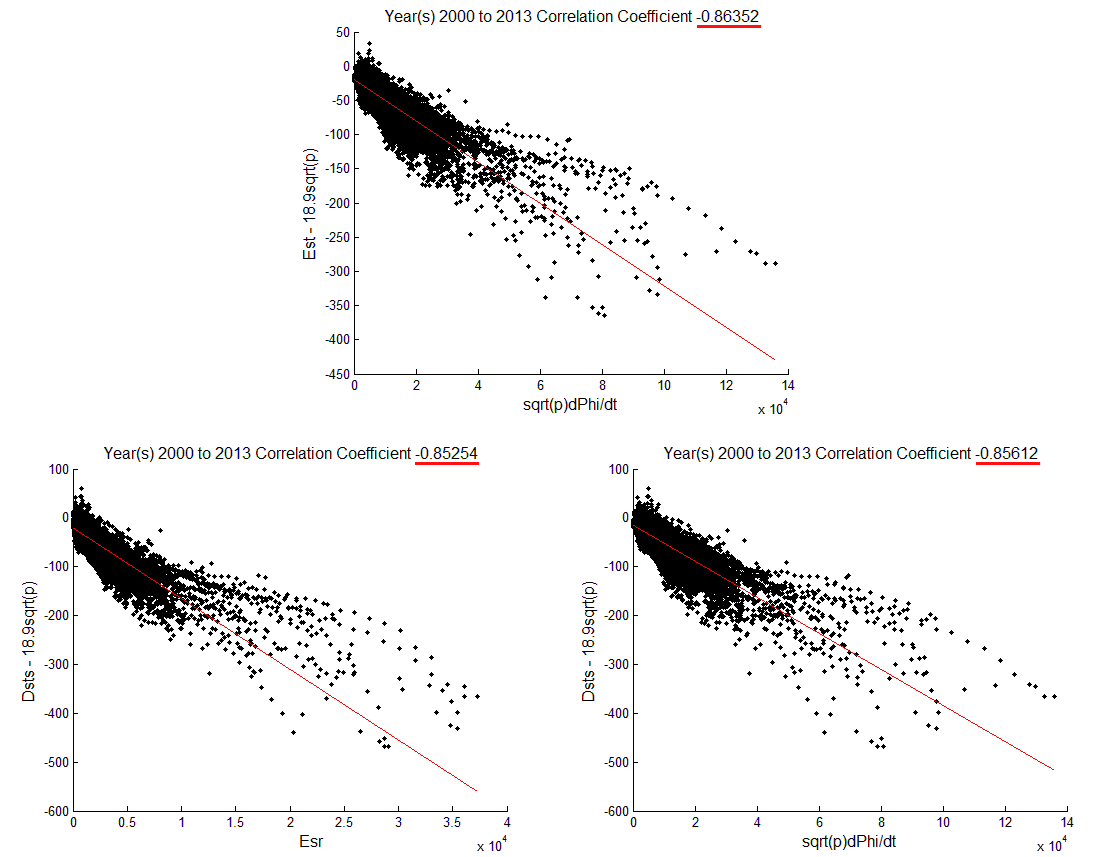
\includegraphics[width=\textwidth]{./dstestscatter}
 \vspace{-15pt}
  \caption{Examples of some output scatter plots. Scatter plots of Est versus $p^{1/2}d\Phi_{MP}/dt$ (top), $Dst$ versus $E_{SR}$ (bottom left), and $Dst$ versus $p^{1/2}d\Phi_{MP}/dt$ (bottom right).} \label{fig:dstestscatter}
  
	\vspace{15pt}
    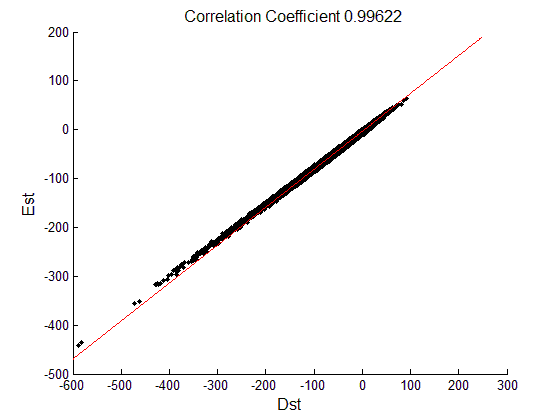
\includegraphics[width=0.8\textwidth]{./estscatter}
 \vspace{-5pt}
  \caption{A scatter plot illustrating that the Dst index correlates very well with the Est index ($r=0.99$). Dst and Est are so well correlated that comparing $p^{1/2}d\Phi/dt$ with Est will never be that much different from comparing it with Dst.} \label{fig:estdst}
 \end{figure} 
 
\begin{figure}
\centering
 \vspace{-20pt}
    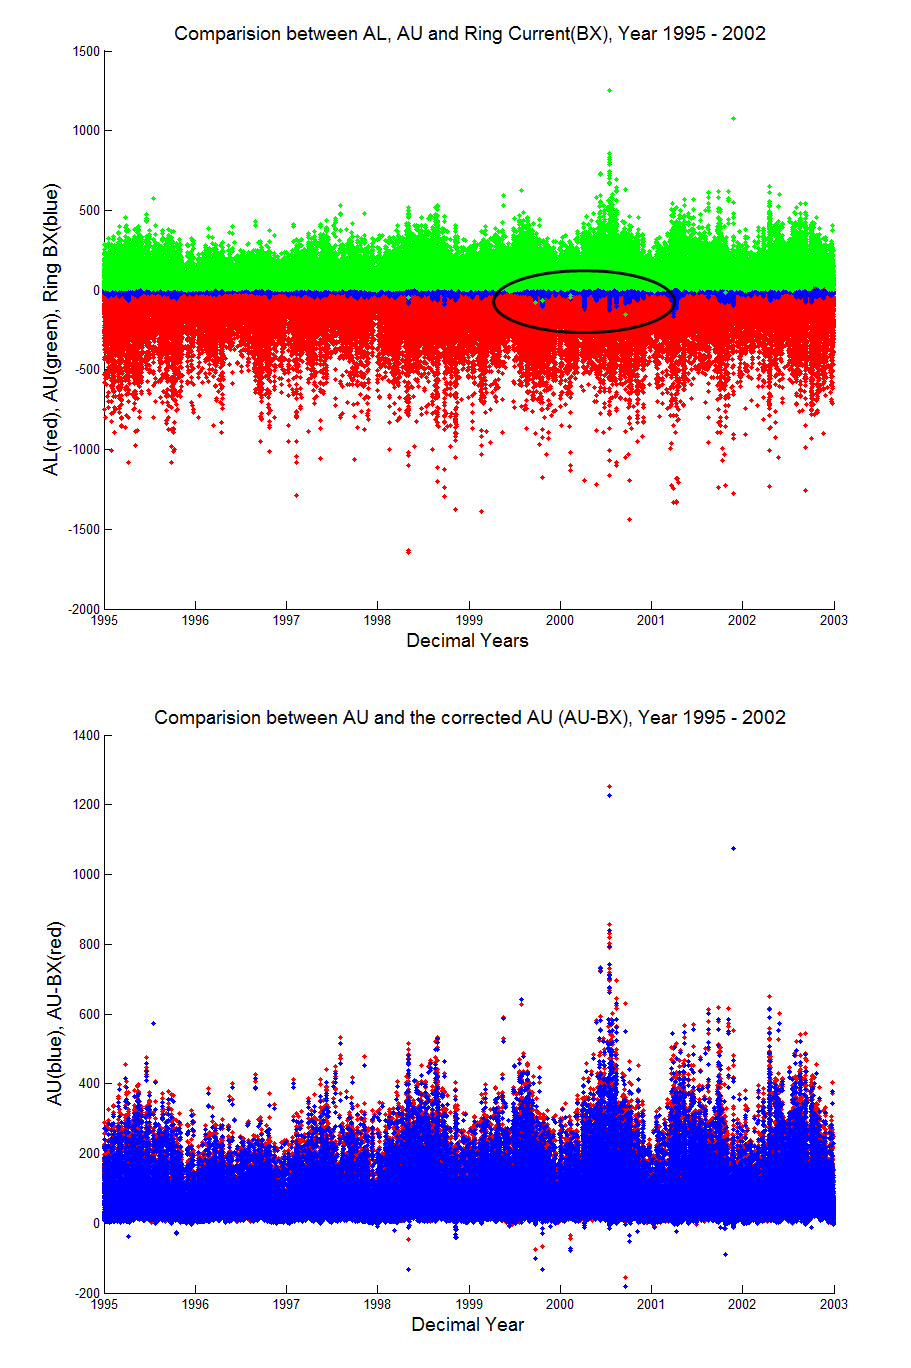
\includegraphics[width=\textwidth]{./comparingAE}
 \vspace{-30pt}
  \caption{Top panel: A time-series scatter plot comparing the AL values (red), AU values (green), and x-component of the Ring Current (blue). The circled area shows that there is a possible correlation between the negative AU values and the x-component of ring current. Bottom panel: A times-series scatter plot comparing the AU index values(blue) with the corrected AU index values (red).} \label{fig:comparingAE}
 \end{figure} 

\chapter{Discussion and Conclusion}\label{chap:discussion}


\cite{newell07} was only interested in the correlation coefficients from the plots, such as those shown in Figure~\ref{fig:dstestscatter}, but the (red) best-fit lines on those correlation plots could be used to predict the Dst/Est/AU/AL from solar wind parameters. The `Gradient' and the `Y-intercept' are presented in Table~\ref{tab:result}. The indices prediction could be done by using the gradient to scale down the x-axis (coupling functions) and apply an offset (y-intercept) to determine the index value on the y-axis.

Regardless of the exact values, the difference between ${p^{1/2}d\Phi_{MP}/dt}$ and $E_{SR}$ for the 1995-2002 Dst data in the study by \cite{newell07} is very small. It is possible that what \cite{newell07}is arguing is that their coupling function, $d\Phi_{MP}/dt$, is the best coupling function across all the indices they studied. However, the analysis from this investigation does not seem to support this claim since the the correlations between $d\Phi_{MP}/dt$ and Dst, Est, AU, and AL appear to be very inconsistent.  

This project proposed and investigated the hypothesis that magnetic disturbances can be better predicted by replacing the Dst index with the Est index. The hypothesis is true for the coupling function $p^{1/2}d\Phi_{MP}/dt$, however, this is not the case for the coupling function $E_{SR}$. Once the Dst index is replaced with the Est index, the correlation coefficients produced from the 1995-2002 and 2000-2013 data are lower than before the replacement.The first conjecture was the possibility of the $E_{SR}$ function having different solar wind integration time (Table~\ref{tab:inttable}) from the ${p^{1/2}d\Phi_{MP}/dt}$ function. However, the time integration was done after the calculation of the coupling functions, which means that the the optimization of the solar wind parameters and the optimization of the coupling functions are two independent operations. Therefore, the integration time should not be specific to a particular coupling function.

However, after all the corrections and using more recent data from 2000-2013, the coupling function ${p^{1/2}d\Phi_{MP}/dt}$ produced higher correlation coefficients than the coupling function $E_{SR}$, overall. The difference is very small which is due to the fact that Est and Dst are extremely well correlated ($r=0.99$), even if they can differ slightly in amplitude. So, when correlating with Solar Wind parameters, any improvement will be small compared to the failings of the coupling function ($r  \approx 0.85$). It is, nevertheless, an improvement on the prediction model. Therefore, it can be used to support our hypothesis that better prediction of the magnetic disturbances could be done by replacing the Dst index with the Est index, which correlates better with solar wind parameters, through the coupling function, ${p^{1/2}d\Phi_{MP}/dt}$. 

Regarding the results from the correlation between the AU and AL indices with the coupling function $d\Phi_{MP}/dt$ (Table~\ref{tab:result}), it was found that roughly $8\%$ of the AU index and $6\%$ of the AL index were the contribution from the x-component of the ring current. However, it can be said that the correction improved the correlation for the AU index, but was not so for the AL index. Overall, the improvement in the AU index is quantitatively better than the worsening of the AL index. 

All of the factors that went into calculating the coupling functions proposed by \cite{newell07} were fine-tuned, some through trial and error, to be optimal for the indices values they used. However, in this study, many magnetic indices were corrected, therefore, the factors which had been optimized for uncorrected values may not have worked as well. 

If more time was available I would like to extend this investigation across more indices, in order to really test \cite{newell07}'s claims. Also, I would like to focus on just one complete solar cycle and investigate the seasonal effect on the AU index. From the bottom panel of Figure~\ref{fig:comparingAE}, it can be seen that the AU values are at maximum around the middle of the year while at minimum around the end and the beginning of each year. It would be interesting to see whether these trends occur recursively and can be predicted. If the trends are there, then how do they affect the prediction model. For example, the ability to predict might work better at some points in the solar cycle than other.


\section*{Acknowledgement}
I offer my sincerest gratitude to my project supervisor, Dr. Brian Hamilton, for his advice and guidance throughout the period of this project. I would also like to thank Helen Le-Mar for proofreading the final draft of the report.






\begin{thebibliography}{9}

\bibitem[Biktash, 2012]{bik12} Biktash, L. (2012), ``Statistical Study of Solar Wind Parameters and Evolution of Dst Variations during $19-23$ Solar Cycles in Relation with Cosmic Ray Variations'', \textit{Sun and Geosphere, vol.7, no.1}, pp.41-44.

\bibitem[Burton \textit{et al}., 1975]{burton75}Burton, R. K., R. L. McPherron, and C. T. Russell. (1975), ``An empirical relationship between interplanetary conditions and Dst'', \textit{J. Geophys. Res., 80(31)}, pp.4204-4214, doi:10.1029/JA080i031p04204.

\bibitem[Campbell, 2003]{campbell03} Campbell, W. H. (2003), ``Introduction to geomagnetic fields'', 2\textsuperscript{nd} ed, \textit{Cambridge: Cambridge University Press}, pp.111-188.

\bibitem[Chapman and Ferraro, 1931]{chapfer31} Chapman, S., and V. C. A. Ferraro. (1931), ``A new theory of magnetic storms'', \textit{Terr. Magn. Atmos. Electr., 36(3)}, pp.171-186, doi:10.1029/TE036i003p00171.

\bibitem[Davis and Sugiura, 1966]{davis66} Davis, T. N., and M. Sugiura. 1966, ``Auroral electrojet activity index AE and its universal time variations'', \textit{J. Geophys. Res., 71(3)}, pp. 785–801, doi:10.1029/JZ071i003p00785.

 \bibitem[Dungey, 1961]{dun61}Dungey, J. W. (1961), ``Interplanetary Magnetic Field and the Auroral Zones", \textit{Phys. Rev. Let., 6}, pp.47-49.

\bibitem[Le \textit{et al}., 2004]{le04}Le, G., C. T. Russell, and K. Takahashi (2004), ``Morphology of the ring current derived from magnetic field observations'', \textit{Ann. Geophys., 22}, pp.1267-1295, doi:10.5194/angeo-22-1267-2004.

\bibitem[Maus and Weidelt, 2004]{maus04} Maus, S., and P. Weidelt. (2004), ``Separating the magnetospheric disturbance magnetic field into external and transient internal contributions using a 1D conductivity model of the Earth'', \textit{Geophys. Res. Lett., 31}, L12614, doi:10.1029/2004GL020232.

\bibitem[McPherron, 1995]{mcpher95} McPherron, R. L. (1995), ``Magnetospheric Dynamics'', In: Kivelson M. G. and Russel, C. T. (eds) Introduction to space physics, \textit{Cambridge University Press, New York, USA}, pp.400-458.

\bibitem[Menvielle \textit{et al}., 2011]{men11}Menvielle, M, T. Iyemori, A. Marchaudon, and M. Nosé (2011), ``Geomagnetic Indices'', In: M. Mandea and M. Korte (eds.) Geomagnetic Observations and Models, \textit{Springer Netherlands}, pp.183-228, doi:10.1007/978-90-481-9858-0\_8.

\bibitem[Newell \textit{et al}., 2007]{newell07} Newell, P., T. Sotirelis, K. Liou,  C. Meng,  and F. Rich. (2007), ``A nearly universal solar wind-magnetosphere coupling function inferred from 10 magnetospheric state variables'', \textit{J. Geophys. Res., 112}, A01206, doi:10.1029/2006JA012015.

\bibitem[Russell , 1972a]{russell72}Russell, C. T. (1972a), "The configuration of the magnetosphere", In: E. R. Dyer (ed.), Critical Problems of Magnetospheric Physics, \textit{IUCSTP Secretariat, National Academy of Sciences, Washington}, pp. 1.

\bibitem[Russell, 2000]{russell00} Russell, C.T. (2000), "The solar wind interaction with the Earth's magnetosphere: a tutorial'', \textit{Plasma Science, IEEE Transactions on}, vol.28, no.6, pp.1818-1830, doi:10.1109/27.902211

\bibitem[Russell \textit{et al}., 1974]{russell74} Russell, T., R.L. McPherron, and R.K. Burton. (1974), ``On the cause of geomagnetic storms'', \textit{J. Geophys. Res., 79(7)}, pp.1105-1109.

\bibitem[Scurry and Russell, 1991]{scurry91}Scurry, L., and C. T. Russell. (1991), ``Proxy studies of energy transfer to the magnetosphere'', \textit{J. Geophys. Res., 96(A6)}, pp.9541-9548, doi:10.1029/91JA00569.\

\bibitem[Sugiura and Kamei, 1991]{sugi91} Sugiura, M., and Kamei, T. (1991), ``Equatorial Dst index'', \textit{IAGA Bulletin}, No.40, pp.1957-1986.

\bibitem[Utada et al, 2003]{utada03} Utada, H., T. Koyama, H. Shimizu, and A. D. Chave. (2003), ``A semi-global reference model foe electrical model for electrical conductivity in the mid-mantle beneath the north Pacific region'', \textit{Geophys. Res. Lett., 30(4)}, 1194, doi:10.1029/2002GL016092.
\end{thebibliography}



\appendix
\chapter{Main MATLAB\textsuperscript{\textregistered} code} \label{chap:app}
\vspace{-15pt}
\lstset{language=Matlab,%
    %basicstyle=\color{red},
    breaklines=true,%
    morekeywords={matlab2tikz},
    keywordstyle=\color{blue},%
    morekeywords=[2]{1}, keywordstyle=[2]{\color{black}},
    identifierstyle=\color{black},%
    stringstyle=\color{mylilas},
    commentstyle=\color{mygreen},%
    showstringspaces=false,%without this there will be a symbol in the places where there is a space
    numbers=left,%
    numberstyle={\tiny \color{black}},% size of the numbers
    numbersep=9pt, % this defines how far the numbers are from the text
    emph=[1]{for,end,break},emphstyle=[1]\color{red}, %some words to emphasise
    %emph=[2]{word1,word2}, emphstyle=[2]{style},   
}

\lstinputlisting{dPhiCode.m}



\end{document}
